\begin{answer}

\begin{figure}[H]
    \centering
    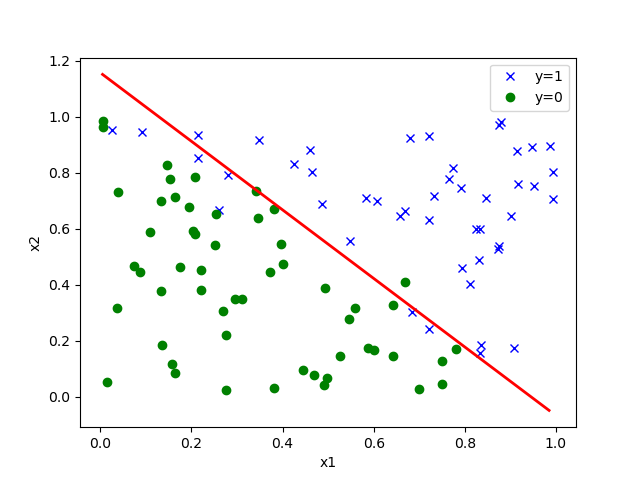
\includegraphics[width=0.5\linewidth]{logreg_pred_a_reg.png}
    \caption{ps2::q3::(d)\_ds1\_a\_reg}
    \label{fig:enter-label}
\end{figure}

\begin{figure}[H]
    \centering
    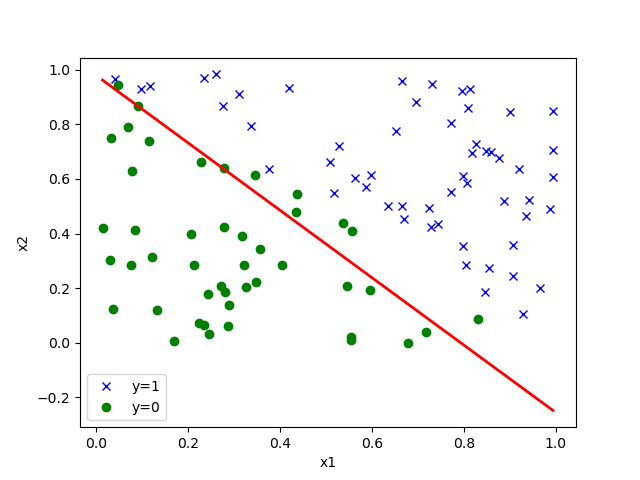
\includegraphics[width=0.5\linewidth]{logreg_pred_b_reg.png}
    \caption{ps2::q3::(d)\_ds1\_b\_reg}
    \label{fig:enter-label}
\end{figure}


Q1: For both datasets, print the final value of $\theta$, and compare it to the final value of $\theta$ without regularization. \\
For dataset a, final theta without regularization = $\left(-20.75421386, 21.39095011, 19.79278897 \right)$, final theta with regularization $\left( -2.54004718, 2.68905075, 2.19522613 \right)$\\

For dataset b, final theta without regularization = $\left(-52.72003622  , 52.90881428, 52.67579144 \right)$, final theta with regularization $\left( -2.33355301, 2.94372417, 2.38236189 \right)$\\

So regularization significantly reduces the magnitude of $\theta$ \\ 


Q2: Additionally, include a plot of the decision boundary and training data for both datasets and comment on the results qualitatively. How does the decision boundary compare to the one obtained without regularization, especially with respect to the worst misclassified example \\ 

For dataset a, final loss without regularization = 0.15987481169737058, final loss with regularization is 0.4081670124984385. The loss doubly increased by introducing regularization and decision boundary changes the output for about 4 samples. The worst misclassfied example are already misclassfied in the training, and newly misclassfied samples stay close to the decision bountry meaning their classification is vague\\

For dataset b, final loss without regularization = 0.03045282298834201, final loss with regularization is 0.36229770962458985. The loss with regularization is 10+ times comparing to the one without. From output, there are 0 vaguely classified samples without regularization, but about 6 to 8 samples are wrongly classified by introducing regularization. The conclusion is, the decision boundary with regularization no longer predicts over-confidently on some value samples, but they still stay close to the decision boundary meaning their class is vague\\ 

Q3: in what cases may this be desirable?

In some cases where the need to convey the vagueness of output is import, we would better use regularization to avoid over-confidently classify samples. Use cases can be diseases diagnose, criminal records classification etc 



\end{answer}
